\section{Correlation analysis with data reduction}

\subsection{Choice between PCA and t-SNE}
We ave a lot of Correlation in our dataset so the usage of PCA is recommanded. We can see on the scree plot that we have to keep 2 components for our analysis.
We can make 2 subsets of our data frame: 1 with the 2 components Temperature and Relative humidity and an other subset with the other components. The Absolute humidity is not used because there isn't any correlation with the other components.
If we keep 2 components (1 of each group) we have more than 95\% of the variance explained. We can see that the 2 components are not correlated with each other. We can use the 2 components for our analysis.
\begin{figure}[h]
\centering
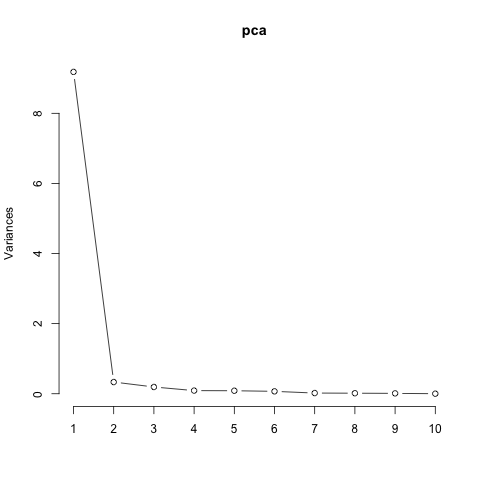
\includegraphics[width=0.5\textwidth]{figs/pca.png}
\caption{Scree plot of the PCA}
\label{fig:scree_plot}
\end{figure}

\subsection{2D plot of the data}

On the graph below we can see the 2 composents of the PCA. We can say that they are not correlated with each other because the arrows are not aligned.
\begin{figure}[H]
\centering
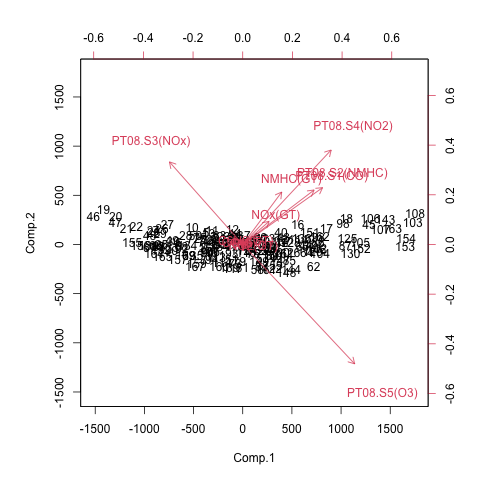
\includegraphics[width=0.8\textwidth]{figs/biplot.png}
\caption{2D plot of the data}
\label{fig:2d_plot}
\end{figure}
